% \chapter{Protokół AISG 2.0}
\subsection{Ramka U}
Jej nazwa pochodzi z języka angielskiego ,,Unnumbered'' co oznacza nienumerowana.\autocite{WIKI_ENG_HDLC}
Wzięło się to z tego, że wielokrotnie wysłana wiadomość tego typu, zawsze posiada tą samą wartość bajtu kontrolnego.
Służy ona do zarządzania warstwą łącza danych, a czasami również do przesyłania pewnych informacji.
\newline
Bajty budujące ramkę:
\begin{itemize}
	\item Adresu;
	\item Kontrolny;
\end{itemize}
Poszczególne wiadomości przesyłane przy pomocy tej ramki identyfikowane są dzięki charakterystycznej wartości bajtu kontrolnego.

\subsection{Ramka I}
Jej nazwa pochodzi z języka angielskiego ,,Information'' co oznacza informacyjna. \autocite{WIKI_ENG_HDLC}
Dzięki niej można żadać od urządzenia podrzędnego wykonania wysokopoziomowej operacji zdefiniowanej przez warstwę aplikacyjną, a nawet przesłać 
najnowszą wersję oprogramowania urządzenia. Jej długość definiowana jest podczas XID negocjacji w trakcie zestawiania warstwy łącza danych. 
\newline
Bajty budujące ramkę:
\begin{itemize}
	\item Adresu;
	\item Kontrolny;
	\item Kodu procedury;
	\item Dodatkowe wartości procedury/raportujące proces wykonania procedury;
\end{itemize}
Wiadomości tego typu przy wielokrotnym zawołaniu żądania wykonania tej samej procedury posiadają zmienną wartość bajtu kontrolnego, co różni ją od ramki U czy XID. 
\newline
Proces ten w przypadku bitu który ustawiany jest na pozycji 4 bajtu kontrolnego P/F\footnote{\label{Bit P/F} P/F - ang. bit Pool/Final} służy do:
\begin{itemize}
	\item Poinformowania urządzenia podrzędnego, że urządzenie nadrzędne żada odpowiedzi na właśnie przesyłaną wiadomość;
	\item Poinformowania urządzenia nadrzędnego o zakończeniu nadawania odpowiedzi na wiadomość;
\end{itemize}
Wartość bitu na pozycji 0 jest zawsze równa 0. 
Bity od piątego do siódmego włącznie definiują nam licznik wiadomości odebranych przez urządzenie nadrzędne czyli N(R)\footnote{\label{N(R)} N(R) - ang. Receive sequence number}. 
Bity od pierwszego do trzeciego włącznie definiują nam licznik wiadomości wysłanych przez urządzenie nadrzędne czyli N(S)\footnote{\label{N(S)} N(S) - ang. Send sequence number}.
Na poniższym diagramie przedstawiono ewaluację bajtu kontrolnego dla kolejnych wiadomości warstwy aplikacyjnej.
\begin{figure}[h!]
\centering
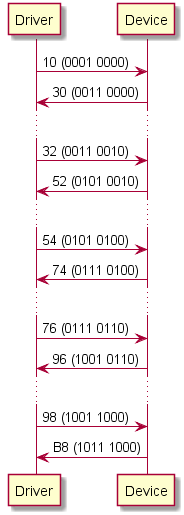
\includegraphics[scale=1.0]{out/FrameI_Bajt_kontrolny/FrameI_Bajt_kontrolny.png}
\caption{Ramka informacyjna - ewaluacja bajtu kontrolnego}
\end{figure}
